\documentclass[1p]{elsarticle_modified}
%\bibliographystyle{elsarticle-num}

%\usepackage[colorlinks]{hyperref}
%\usepackage{abbrmath_seonhwa} %\Abb, \Ascr, \Acal ,\Abf, \Afrak
\usepackage{amsfonts}
\usepackage{amssymb}
\usepackage{amsmath}
\usepackage{amsthm}
\usepackage{scalefnt}
\usepackage{amsbsy}
\usepackage{kotex}
\usepackage{caption}
\usepackage{subfig}
\usepackage{color}
\usepackage{graphicx}
\usepackage{xcolor} %% white, black, red, green, blue, cyan, magenta, yellow
\usepackage{float}
\usepackage{setspace}
\usepackage{hyperref}

\usepackage{tikz}
\usetikzlibrary{arrows}

\usepackage{multirow}
\usepackage{array} % fixed length table
\usepackage{hhline}

%%%%%%%%%%%%%%%%%%%%%
\makeatletter
\renewcommand*\env@matrix[1][\arraystretch]{%
	\edef\arraystretch{#1}%
	\hskip -\arraycolsep
	\let\@ifnextchar\new@ifnextchar
	\array{*\c@MaxMatrixCols c}}
\makeatother %https://tex.stackexchange.com/questions/14071/how-can-i-increase-the-line-spacing-in-a-matrix
%%%%%%%%%%%%%%%

\usepackage[normalem]{ulem}

\newcommand{\msout}[1]{\ifmmode\text{\sout{\ensuremath{#1}}}\else\sout{#1}\fi}
%SOURCE: \msout is \stkout macro in https://tex.stackexchange.com/questions/20609/strikeout-in-math-mode

\newcommand{\cancel}[1]{
	\ifmmode
	{\color{red}\msout{#1}}
	\else
	{\color{red}\sout{#1}}
	\fi
}

\newcommand{\add}[1]{
	{\color{blue}\uwave{#1}}
}

\newcommand{\replace}[2]{
	\ifmmode
	{\color{red}\msout{#1}}{\color{blue}\uwave{#2}}
	\else
	{\color{red}\sout{#1}}{\color{blue}\uwave{#2}}
	\fi
}

\newcommand{\Sol}{\mathcal{S}} %segment
\newcommand{\D}{D} %diagram
\newcommand{\A}{\mathcal{A}} %arc


%%%%%%%%%%%%%%%%%%%%%%%%%%%%%5 test

\def\sl{\operatorname{\textup{SL}}(2,\Cbb)}
\def\psl{\operatorname{\textup{PSL}}(2,\Cbb)}
\def\quan{\mkern 1mu \triangleright \mkern 1mu}

\theoremstyle{definition}
\newtheorem{thm}{Theorem}[section]
\newtheorem{prop}[thm]{Proposition}
\newtheorem{lem}[thm]{Lemma}
\newtheorem{ques}[thm]{Question}
\newtheorem{cor}[thm]{Corollary}
\newtheorem{defn}[thm]{Definition}
\newtheorem{exam}[thm]{Example}
\newtheorem{rmk}[thm]{Remark}
\newtheorem{alg}[thm]{Algorithm}

\newcommand{\I}{\sqrt{-1}}
\begin{document}

%\begin{frontmatter}
%
%\title{Boundary parabolic representations of knots up to 8 crossings}
%
%%% Group authors per affiliation:
%\author{Yunhi Cho} 
%\address{Department of Mathematics, University of Seoul, Seoul, Korea}
%\ead{yhcho@uos.ac.kr}
%
%
%\author{Seonhwa Kim} %\fnref{s_kim}}
%\address{Center for Geometry and Physics, Institute for Basic Science, Pohang, 37673, Korea}
%\ead{ryeona17@ibs.re.kr}
%
%\author{Hyuk Kim}
%\address{Department of Mathematical Sciences, Seoul National University, Seoul 08826, Korea}
%\ead{hyukkim@snu.ac.kr}
%
%\author{Seokbeom Yoon}
%\address{Department of Mathematical Sciences, Seoul National University, Seoul, 08826,  Korea}
%\ead{sbyoon15@snu.ac.kr}
%
%\begin{abstract}
%We find all boundary parabolic representation of knots up to 8 crossings.
%
%\end{abstract}
%\begin{keyword}
%    \MSC[2010] 57M25 
%\end{keyword}
%
%\end{frontmatter}

%\linenumbers
%\tableofcontents
%
\newcommand\colored[1]{\textcolor{white}{\rule[-0.35ex]{0.8em}{1.4ex}}\kern-0.8em\color{red} #1}%
%\newcommand\colored[1]{\textcolor{white}{ #1}\kern-2.17ex	\textcolor{white}{ #1}\kern-1.81ex	\textcolor{white}{ #1}\kern-2.15ex\color{red}#1	}

{\Large $\underline{12n_{0205}~(K12n_{0205})}$}

\setlength{\tabcolsep}{10pt}
\renewcommand{\arraystretch}{1.6}
\vspace{1cm}\begin{tabular}{m{100pt}>{\centering\arraybackslash}m{274pt}}
\multirow{5}{120pt}{
	\centering
	\includegraphics[width=112pt]{../../../GIT/diagram.site/Diagrams/png/2294_12n_0205.png}\\
\ \ \ A knot diagram\footnotemark}&
\allowdisplaybreaks
\textbf{Linearized knot diagam} \\
\cline{2-2}
 &
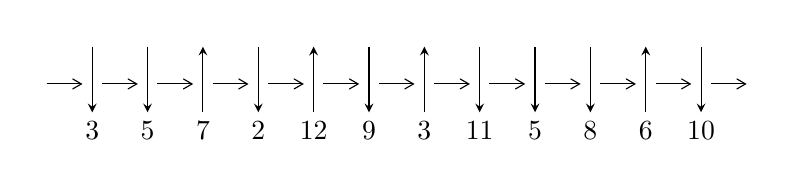
\begin{tikzpicture}[x=20pt, y=17pt]
	% nodes
	\node (C0) at (0, 0) {};
	\node (C1) at (1, 0) {};
	\node (C1U) at (1, +1) {};
	\node (C1D) at (1, -1) {3};

	\node (C2) at (2, 0) {};
	\node (C2U) at (2, +1) {};
	\node (C2D) at (2, -1) {5};

	\node (C3) at (3, 0) {};
	\node (C3U) at (3, +1) {};
	\node (C3D) at (3, -1) {7};

	\node (C4) at (4, 0) {};
	\node (C4U) at (4, +1) {};
	\node (C4D) at (4, -1) {2};

	\node (C5) at (5, 0) {};
	\node (C5U) at (5, +1) {};
	\node (C5D) at (5, -1) {12};

	\node (C6) at (6, 0) {};
	\node (C6U) at (6, +1) {};
	\node (C6D) at (6, -1) {9};

	\node (C7) at (7, 0) {};
	\node (C7U) at (7, +1) {};
	\node (C7D) at (7, -1) {3};

	\node (C8) at (8, 0) {};
	\node (C8U) at (8, +1) {};
	\node (C8D) at (8, -1) {11};

	\node (C9) at (9, 0) {};
	\node (C9U) at (9, +1) {};
	\node (C9D) at (9, -1) {5};

	\node (C10) at (10, 0) {};
	\node (C10U) at (10, +1) {};
	\node (C10D) at (10, -1) {8};

	\node (C11) at (11, 0) {};
	\node (C11U) at (11, +1) {};
	\node (C11D) at (11, -1) {6};

	\node (C12) at (12, 0) {};
	\node (C12U) at (12, +1) {};
	\node (C12D) at (12, -1) {10};
	\node (C13) at (13, 0) {};

	% arrows
	\draw[->,>={angle 60}]
	(C0) edge (C1) (C1) edge (C2) (C2) edge (C3) (C3) edge (C4) (C4) edge (C5) (C5) edge (C6) (C6) edge (C7) (C7) edge (C8) (C8) edge (C9) (C9) edge (C10) (C10) edge (C11) (C11) edge (C12) (C12) edge (C13) ;	\draw[->,>=stealth]
	(C1U) edge (C1D) (C2U) edge (C2D) (C3D) edge (C3U) (C4U) edge (C4D) (C5D) edge (C5U) (C6U) edge (C6D) (C7D) edge (C7U) (C8U) edge (C8D) (C9U) edge (C9D) (C10U) edge (C10D) (C11D) edge (C11U) (C12U) edge (C12D) ;
	\end{tikzpicture} \\
\hhline{~~} \\& 
\textbf{Solving Sequence} \\ \cline{2-2} 
 &
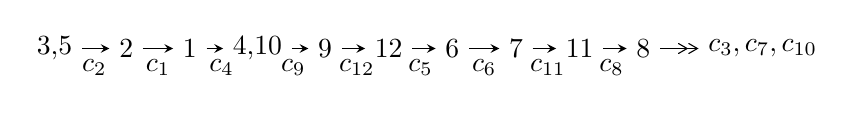
\begin{tikzpicture}[x=23pt, y=7pt]
	% node
	\node (A0) at (-1/8, 0) {3,5};
	\node (A1) at (1, 0) {2};
	\node (A2) at (2, 0) {1};
	\node (A3) at (49/16, 0) {4,10};
	\node (A4) at (33/8, 0) {9};
	\node (A5) at (41/8, 0) {12};
	\node (A6) at (49/8, 0) {6};
	\node (A7) at (57/8, 0) {7};
	\node (A8) at (65/8, 0) {11};
	\node (A9) at (73/8, 0) {8};
	\node (C1) at (1/2, -1) {$c_{2}$};
	\node (C2) at (3/2, -1) {$c_{1}$};
	\node (C3) at (5/2, -1) {$c_{4}$};
	\node (C4) at (29/8, -1) {$c_{9}$};
	\node (C5) at (37/8, -1) {$c_{12}$};
	\node (C6) at (45/8, -1) {$c_{5}$};
	\node (C7) at (53/8, -1) {$c_{6}$};
	\node (C8) at (61/8, -1) {$c_{11}$};
	\node (C9) at (69/8, -1) {$c_{8}$};
	\node (A10) at (11, 0) {$c_{3},c_{7},c_{10}$};

	% edge
	\draw[->,>=stealth]	
	(A0) edge (A1) (A1) edge (A2) (A2) edge (A3) (A3) edge (A4) (A4) edge (A5) (A5) edge (A6) (A6) edge (A7) (A7) edge (A8) (A8) edge (A9) ;
	\draw[->>,>={angle 60}]	
	(A9) edge (A10);
\end{tikzpicture} \\ 

\end{tabular} \\

\footnotetext{
The image of knot diagram is generated by the software ``\textbf{Draw programme}" developed by Andrew Bartholomew(\url{http://www.layer8.co.uk/maths/draw/index.htm\#Running-draw}), where we modified some parts for our purpose(\url{https://github.com/CATsTAILs/LinksPainter}).
}\phantom \\ \newline 
\centering \textbf{Ideals for irreducible components\footnotemark of $X_{\text{par}}$} 
 
\begin{align*}
I^u_{1}&=\langle 
1.70976\times10^{62} u^{52}-3.03954\times10^{60} u^{51}+\cdots+8.90112\times10^{63} b-1.06077\times10^{64},\\
\phantom{I^u_{1}}&\phantom{= \langle  }-1.10028\times10^{63} u^{52}-1.18132\times10^{64} u^{51}+\cdots+9.89014\times10^{62} a-1.33065\times10^{64},\\
\phantom{I^u_{1}}&\phantom{= \langle  }u^{53}+11 u^{52}+\cdots+27 u+1\rangle \\
I^u_{2}&=\langle 
a^6+2 a^4+3 a^2+b+2,\;a^9- a^8+2 a^7- a^6+3 a^5- a^4+2 a^3+a+1,\;u-1\rangle \\
I^u_{3}&=\langle 
u^5+4 u^4+3 u^3-2 u^2+3 b-3 u-1,\;a,\;u^6+u^5- u^4-2 u^3+u+1\rangle \\
\\
\end{align*}
\raggedright * 3 irreducible components of $\dim_{\mathbb{C}}=0$, with total 68 representations.\\
\footnotetext{All coefficients of polynomials are rational numbers. But the coefficients are sometimes approximated in decimal forms when there is not enough margin.}
\newpage
\renewcommand{\arraystretch}{1}
\centering \section*{I. $I^u_{1}= \langle 1.71\times10^{62} u^{52}-3.04\times10^{60} u^{51}+\cdots+8.90\times10^{63} b-1.06\times10^{64},\;-1.10\times10^{63} u^{52}-1.18\times10^{64} u^{51}+\cdots+9.89\times10^{62} a-1.33\times10^{64},\;u^{53}+11 u^{52}+\cdots+27 u+1 \rangle$}
\flushleft \textbf{(i) Arc colorings}\\
\begin{tabular}{m{7pt} m{180pt} m{7pt} m{180pt} }
\flushright $a_{3}=$&$\begin{pmatrix}1\\0\end{pmatrix}$ \\
\flushright $a_{5}=$&$\begin{pmatrix}0\\u\end{pmatrix}$ \\
\flushright $a_{2}=$&$\begin{pmatrix}1\\- u^2\end{pmatrix}$ \\
\flushright $a_{1}=$&$\begin{pmatrix}- u^2+1\\- u^2\end{pmatrix}$ \\
\flushright $a_{4}=$&$\begin{pmatrix}u\\- u^3+u\end{pmatrix}$ \\
\flushright $a_{10}=$&$\begin{pmatrix}1.11250 u^{52}+11.9444 u^{51}+\cdots+116.277 u+13.4543\\-0.0192084 u^{52}+0.000341478 u^{51}+\cdots+15.5915 u+1.19173\end{pmatrix}$ \\
\flushright $a_{9}=$&$\begin{pmatrix}1.11250 u^{52}+11.9444 u^{51}+\cdots+116.277 u+13.4543\\-0.382334 u^{52}-3.37450 u^{51}+\cdots+8.79186 u+0.898684\end{pmatrix}$ \\
\flushright $a_{12}=$&$\begin{pmatrix}-0.851461 u^{52}-9.05934 u^{51}+\cdots-65.4023 u-7.59764\\0.902652 u^{52}+8.13404 u^{51}+\cdots+10.0567 u-0.0126855\end{pmatrix}$ \\
\flushright $a_{6}=$&$\begin{pmatrix}-0.0355732 u^{52}-0.584596 u^{51}+\cdots+13.1513 u-0.387998\\0.349645 u^{52}+3.23765 u^{51}+\cdots+1.90889 u+0.0261483\end{pmatrix}$ \\
\flushright $a_{7}=$&$\begin{pmatrix}0.130529 u^{52}+1.68645 u^{51}+\cdots+35.4466 u+5.88903\\0.154225 u^{52}+1.43278 u^{51}+\cdots+4.53267 u+0.381154\end{pmatrix}$ \\
\flushright $a_{11}=$&$\begin{pmatrix}-0.284754 u^{52}-3.11922 u^{51}+\cdots-39.9792 u-6.27018\\0.427550 u^{52}+3.88507 u^{51}+\cdots-1.47440 u-0.445947\end{pmatrix}$ \\
\flushright $a_{8}=$&$\begin{pmatrix}0.284754 u^{52}+3.11922 u^{51}+\cdots+39.9792 u+6.27018\\0.154225 u^{52}+1.43278 u^{51}+\cdots+4.53267 u+0.381154\end{pmatrix}$\\&\end{tabular}
\flushleft \textbf{(ii) Obstruction class $= -1$}\\~\\
\flushleft \textbf{(iii) Cusp Shapes $= -0.225150 u^{52}-2.33690 u^{51}+\cdots-27.9440 u-9.85542$}\\~\\
\newpage\renewcommand{\arraystretch}{1}
\flushleft \textbf{(iv) u-Polynomials at the component}\newline \\
\begin{tabular}{m{50pt}|m{274pt}}
Crossings & \hspace{64pt}u-Polynomials at each crossing \\
\hline $$\begin{aligned}c_{1}\end{aligned}$$&$\begin{aligned}
&u^{53}+63 u^{52}+\cdots+371 u+1
\end{aligned}$\\
\hline $$\begin{aligned}c_{2},c_{4}\end{aligned}$$&$\begin{aligned}
&u^{53}-11 u^{52}+\cdots+27 u-1
\end{aligned}$\\
\hline $$\begin{aligned}c_{3},c_{7}\end{aligned}$$&$\begin{aligned}
&u^{53}-2 u^{52}+\cdots+2560 u+512
\end{aligned}$\\
\hline $$\begin{aligned}c_{5},c_{11}\end{aligned}$$&$\begin{aligned}
&u^{53}+3 u^{52}+\cdots+3 u+1
\end{aligned}$\\
\hline $$\begin{aligned}c_{6}\end{aligned}$$&$\begin{aligned}
&9(9 u^{53}-30 u^{52}+\cdots-9820 u-5144)
\end{aligned}$\\
\hline $$\begin{aligned}c_{8},c_{10}\end{aligned}$$&$\begin{aligned}
&u^{53}-8 u^{52}+\cdots+936 u-81
\end{aligned}$\\
\hline $$\begin{aligned}c_{9}\end{aligned}$$&$\begin{aligned}
&u^{53}+2 u^{52}+\cdots+22464 u-5184
\end{aligned}$\\
\hline $$\begin{aligned}c_{12}\end{aligned}$$&$\begin{aligned}
&9(9 u^{53}-6 u^{52}+\cdots+279223 u-329)
\end{aligned}$\\
\hline
\end{tabular}\\~\\
\newpage\renewcommand{\arraystretch}{1}
\flushleft \textbf{(v) Riley Polynomials at the component}\newline \\
\begin{tabular}{m{50pt}|m{274pt}}
Crossings & \hspace{64pt}Riley Polynomials at each crossing \\
\hline $$\begin{aligned}c_{1}\end{aligned}$$&$\begin{aligned}
&y^{53}-135 y^{52}+\cdots+162995 y-1
\end{aligned}$\\
\hline $$\begin{aligned}c_{2},c_{4}\end{aligned}$$&$\begin{aligned}
&y^{53}-63 y^{52}+\cdots+371 y-1
\end{aligned}$\\
\hline $$\begin{aligned}c_{3},c_{7}\end{aligned}$$&$\begin{aligned}
&y^{53}+54 y^{52}+\cdots+6815744 y-262144
\end{aligned}$\\
\hline $$\begin{aligned}c_{5},c_{11}\end{aligned}$$&$\begin{aligned}
&y^{53}+37 y^{52}+\cdots+11 y-1
\end{aligned}$\\
\hline $$\begin{aligned}c_{6}\end{aligned}$$&$\begin{aligned}
&81(81 y^{53}-3132 y^{52}+\cdots+2.63839\times10^{8} y-2.64607\times10^{7})
\end{aligned}$\\
\hline $$\begin{aligned}c_{8},c_{10}\end{aligned}$$&$\begin{aligned}
&y^{53}-54 y^{52}+\cdots+624672 y-6561
\end{aligned}$\\
\hline $$\begin{aligned}c_{9}\end{aligned}$$&$\begin{aligned}
&y^{53}-36 y^{52}+\cdots-140341248 y-26873856
\end{aligned}$\\
\hline $$\begin{aligned}c_{12}\end{aligned}$$&$\begin{aligned}
&81(81 y^{53}-4590 y^{52}+\cdots+7.81268\times10^{10} y-108241)
\end{aligned}$\\
\hline
\end{tabular}\\~\\
\newpage\flushleft \textbf{(vi) Complex Volumes and Cusp Shapes}
$$\begin{array}{c|c|c}  
\text{Solutions to }I^u_{1}& \I (\text{vol} + \sqrt{-1}CS) & \text{Cusp shape}\\
 \hline 
\begin{aligned}
u &= \phantom{-}0.740987 + 0.599213 I \\
a &= \phantom{-}1.57596 - 0.73751 I \\
b &= \phantom{-}0.321377 - 0.617776 I\end{aligned}
 & -4.33713 - 4.43867 I & -10.24927 + 6.85756 I \\ \hline\begin{aligned}
u &= \phantom{-}0.740987 - 0.599213 I \\
a &= \phantom{-}1.57596 + 0.73751 I \\
b &= \phantom{-}0.321377 + 0.617776 I\end{aligned}
 & -4.33713 + 4.43867 I & -10.24927 - 6.85756 I \\ \hline\begin{aligned}
u &= \phantom{-}1.029610 + 0.245825 I \\
a &= \phantom{-}0.125397 + 0.344874 I \\
b &= \phantom{-}0.310362 + 0.858643 I\end{aligned}
 & -2.07856 - 0.90512 I & \phantom{-0.000000 } 0 \\ \hline\begin{aligned}
u &= \phantom{-}1.029610 - 0.245825 I \\
a &= \phantom{-}0.125397 - 0.344874 I \\
b &= \phantom{-}0.310362 - 0.858643 I\end{aligned}
 & -2.07856 + 0.90512 I & \phantom{-0.000000 } 0 \\ \hline\begin{aligned}
u &= \phantom{-}1.014220 + 0.368097 I \\
a &= \phantom{-}0.17089 + 1.53157 I \\
b &= \phantom{-}1.88007 - 0.54448 I\end{aligned}
 & -7.18708 - 1.12498 I & -14.8807 + 0. I\phantom{ +0.000000I} \\ \hline\begin{aligned}
u &= \phantom{-}1.014220 - 0.368097 I \\
a &= \phantom{-}0.17089 - 1.53157 I \\
b &= \phantom{-}1.88007 + 0.54448 I\end{aligned}
 & -7.18708 + 1.12498 I & -14.8807 + 0. I\phantom{ +0.000000I} \\ \hline\begin{aligned}
u &= \phantom{-}1.14783\phantom{ +0.000000I} \\
a &= \phantom{-}0.526566\phantom{ +0.000000I} \\
b &= \phantom{-}2.18865\phantom{ +0.000000I}\end{aligned}
 & -2.44483\phantom{ +0.000000I} & \phantom{-0.000000 } 0 \\ \hline\begin{aligned}
u &= \phantom{-}0.822832 + 0.202810 I \\
a &= \phantom{-}0.184579 - 0.579850 I \\
b &= \phantom{-}0.34533 + 2.28724 I\end{aligned}
 & -3.14584 - 0.60875 I & -6.43020 - 7.79756 I \\ \hline\begin{aligned}
u &= \phantom{-}0.822832 - 0.202810 I \\
a &= \phantom{-}0.184579 + 0.579850 I \\
b &= \phantom{-}0.34533 - 2.28724 I\end{aligned}
 & -3.14584 + 0.60875 I & -6.43020 + 7.79756 I \\ \hline\begin{aligned}
u &= -0.724671 + 0.356426 I \\
a &= -0.056116 + 0.976114 I \\
b &= \phantom{-}0.178762 + 0.417119 I\end{aligned}
 & \phantom{-}0.78284 - 1.50580 I & \phantom{-}1.85337 + 3.47450 I\\
 \hline 
 \end{array}$$\newpage$$\begin{array}{c|c|c}  
\text{Solutions to }I^u_{1}& \I (\text{vol} + \sqrt{-1}CS) & \text{Cusp shape}\\
 \hline 
\begin{aligned}
u &= -0.724671 - 0.356426 I \\
a &= -0.056116 - 0.976114 I \\
b &= \phantom{-}0.178762 - 0.417119 I\end{aligned}
 & \phantom{-}0.78284 + 1.50580 I & \phantom{-}1.85337 - 3.47450 I \\ \hline\begin{aligned}
u &= \phantom{-}1.229490 + 0.119531 I \\
a &= -1.077010 + 0.000602 I \\
b &= -2.50917 + 2.03905 I\end{aligned}
 & -5.64518 + 2.18249 I & \phantom{-0.000000 } 0 \\ \hline\begin{aligned}
u &= \phantom{-}1.229490 - 0.119531 I \\
a &= -1.077010 - 0.000602 I \\
b &= -2.50917 - 2.03905 I\end{aligned}
 & -5.64518 - 2.18249 I & \phantom{-0.000000 } 0 \\ \hline\begin{aligned}
u &= \phantom{-}0.578578 + 0.484586 I \\
a &= -1.018420 + 0.280436 I \\
b &= -0.415921 + 0.414378 I\end{aligned}
 & -0.90481 - 1.57510 I & -3.08858 + 5.02134 I \\ \hline\begin{aligned}
u &= \phantom{-}0.578578 - 0.484586 I \\
a &= -1.018420 - 0.280436 I \\
b &= -0.415921 - 0.414378 I\end{aligned}
 & -0.90481 + 1.57510 I & -3.08858 - 5.02134 I \\ \hline\begin{aligned}
u &= -0.708934 + 0.120407 I \\
a &= -0.92683 - 1.44462 I \\
b &= -0.469500 - 0.468379 I\end{aligned}
 & -4.72794 - 6.87040 I & -1.05460 + 3.48446 I \\ \hline\begin{aligned}
u &= -0.708934 - 0.120407 I \\
a &= -0.92683 + 1.44462 I \\
b &= -0.469500 + 0.468379 I\end{aligned}
 & -4.72794 + 6.87040 I & -1.05460 - 3.48446 I \\ \hline\begin{aligned}
u &= -1.188110 + 0.522041 I \\
a &= -0.065515 - 0.516096 I \\
b &= -0.181732 - 0.422617 I\end{aligned}
 & -1.55881 + 5.25423 I & \phantom{-0.000000 } 0 \\ \hline\begin{aligned}
u &= -1.188110 - 0.522041 I \\
a &= -0.065515 + 0.516096 I \\
b &= -0.181732 + 0.422617 I\end{aligned}
 & -1.55881 - 5.25423 I & \phantom{-0.000000 } 0 \\ \hline\begin{aligned}
u &= \phantom{-}0.713723 + 1.108540 I \\
a &= -1.145180 + 0.691529 I \\
b &= -1.004520 + 0.127758 I\end{aligned}
 & -11.4354 - 9.7069 I & \phantom{-0.000000 } 0\\
 \hline 
 \end{array}$$\newpage$$\begin{array}{c|c|c}  
\text{Solutions to }I^u_{1}& \I (\text{vol} + \sqrt{-1}CS) & \text{Cusp shape}\\
 \hline 
\begin{aligned}
u &= \phantom{-}0.713723 - 1.108540 I \\
a &= -1.145180 - 0.691529 I \\
b &= -1.004520 - 0.127758 I\end{aligned}
 & -11.4354 + 9.7069 I & \phantom{-0.000000 } 0 \\ \hline\begin{aligned}
u &= \phantom{-}0.645363 + 1.159150 I \\
a &= -0.411472 + 1.090720 I \\
b &= -0.475717 + 0.405091 I\end{aligned}
 & -11.21080 + 2.39200 I & \phantom{-0.000000 } 0 \\ \hline\begin{aligned}
u &= \phantom{-}0.645363 - 1.159150 I \\
a &= -0.411472 - 1.090720 I \\
b &= -0.475717 - 0.405091 I\end{aligned}
 & -11.21080 - 2.39200 I & \phantom{-0.000000 } 0 \\ \hline\begin{aligned}
u &= \phantom{-}0.536755 + 0.402568 I \\
a &= \phantom{-}0.923406 - 0.659788 I \\
b &= \phantom{-}0.89484 - 1.39101 I\end{aligned}
 & -3.70920 + 0.68240 I & -10.13112 + 2.63548 I \\ \hline\begin{aligned}
u &= \phantom{-}0.536755 - 0.402568 I \\
a &= \phantom{-}0.923406 + 0.659788 I \\
b &= \phantom{-}0.89484 + 1.39101 I\end{aligned}
 & -3.70920 - 0.68240 I & -10.13112 - 2.63548 I \\ \hline\begin{aligned}
u &= \phantom{-}0.709864 + 1.162520 I \\
a &= \phantom{-}0.713217 - 0.733177 I \\
b &= \phantom{-}0.685394 - 0.156529 I\end{aligned}
 & -6.83584 - 3.76717 I & \phantom{-0.000000 } 0 \\ \hline\begin{aligned}
u &= \phantom{-}0.709864 - 1.162520 I \\
a &= \phantom{-}0.713217 + 0.733177 I \\
b &= \phantom{-}0.685394 + 0.156529 I\end{aligned}
 & -6.83584 + 3.76717 I & \phantom{-0.000000 } 0 \\ \hline\begin{aligned}
u &= -0.190058 + 0.453543 I \\
a &= -1.217760 + 0.413382 I \\
b &= -0.101388 + 0.374695 I\end{aligned}
 & \phantom{-}1.01456 - 1.24993 I & \phantom{-}3.91266 + 3.38096 I \\ \hline\begin{aligned}
u &= -0.190058 - 0.453543 I \\
a &= -1.217760 - 0.413382 I \\
b &= -0.101388 - 0.374695 I\end{aligned}
 & \phantom{-}1.01456 + 1.24993 I & \phantom{-}3.91266 - 3.38096 I \\ \hline\begin{aligned}
u &= -1.63891 + 0.08655 I \\
a &= -0.523277 - 0.000961 I \\
b &= -2.42482 - 0.70129 I\end{aligned}
 & -11.54620 + 0.81534 I & \phantom{-0.000000 } 0\\
 \hline 
 \end{array}$$\newpage$$\begin{array}{c|c|c}  
\text{Solutions to }I^u_{1}& \I (\text{vol} + \sqrt{-1}CS) & \text{Cusp shape}\\
 \hline 
\begin{aligned}
u &= -1.63891 - 0.08655 I \\
a &= -0.523277 + 0.000961 I \\
b &= -2.42482 + 0.70129 I\end{aligned}
 & -11.54620 - 0.81534 I & \phantom{-0.000000 } 0 \\ \hline\begin{aligned}
u &= -1.65289 + 0.15939 I \\
a &= \phantom{-}0.875260 - 0.410425 I \\
b &= \phantom{-}2.21311 - 0.23469 I\end{aligned}
 & -8.77075 + 4.08365 I & \phantom{-0.000000 } 0 \\ \hline\begin{aligned}
u &= -1.65289 - 0.15939 I \\
a &= \phantom{-}0.875260 + 0.410425 I \\
b &= \phantom{-}2.21311 + 0.23469 I\end{aligned}
 & -8.77075 - 4.08365 I & \phantom{-0.000000 } 0 \\ \hline\begin{aligned}
u &= -1.70501 + 0.03615 I \\
a &= -0.395981 - 0.689977 I \\
b &= -1.41927 + 0.04910 I\end{aligned}
 & -12.33890 + 1.47775 I & \phantom{-0.000000 } 0 \\ \hline\begin{aligned}
u &= -1.70501 - 0.03615 I \\
a &= -0.395981 + 0.689977 I \\
b &= -1.41927 - 0.04910 I\end{aligned}
 & -12.33890 - 1.47775 I & \phantom{-0.000000 } 0 \\ \hline\begin{aligned}
u &= -1.70201 + 0.18739 I \\
a &= -1.42791 + 0.60902 I \\
b &= -2.95092 + 0.61814 I\end{aligned}
 & -12.9006 + 7.5876 I & \phantom{-0.000000 } 0 \\ \hline\begin{aligned}
u &= -1.70201 - 0.18739 I \\
a &= -1.42791 - 0.60902 I \\
b &= -2.95092 - 0.61814 I\end{aligned}
 & -12.9006 - 7.5876 I & \phantom{-0.000000 } 0 \\ \hline\begin{aligned}
u &= -0.276292 + 0.038780 I \\
a &= \phantom{-}3.14779 - 2.19159 I \\
b &= \phantom{-}0.509597 - 0.650771 I\end{aligned}
 & -1.03321 + 2.55519 I & \phantom{-}0.02559 - 3.47308 I \\ \hline\begin{aligned}
u &= -0.276292 - 0.038780 I \\
a &= \phantom{-}3.14779 + 2.19159 I \\
b &= \phantom{-}0.509597 + 0.650771 I\end{aligned}
 & -1.03321 - 2.55519 I & \phantom{-}0.02559 + 3.47308 I \\ \hline\begin{aligned}
u &= \phantom{-}1.73015 + 0.03085 I \\
a &= \phantom{-}0.952566 - 0.310448 I \\
b &= \phantom{-}2.31647 - 0.61550 I\end{aligned}
 & -13.7945 + 6.0358 I & \phantom{-0.000000 } 0\\
 \hline 
 \end{array}$$\newpage$$\begin{array}{c|c|c}  
\text{Solutions to }I^u_{1}& \I (\text{vol} + \sqrt{-1}CS) & \text{Cusp shape}\\
 \hline 
\begin{aligned}
u &= \phantom{-}1.73015 - 0.03085 I \\
a &= \phantom{-}0.952566 + 0.310448 I \\
b &= \phantom{-}2.31647 + 0.61550 I\end{aligned}
 & -13.7945 - 6.0358 I & \phantom{-0.000000 } 0 \\ \hline\begin{aligned}
u &= -1.69334 + 0.39921 I \\
a &= \phantom{-}1.073220 - 0.496311 I \\
b &= \phantom{-}2.64306 - 0.19760 I\end{aligned}
 & -19.2132 + 15.4269 I & \phantom{-0.000000 } 0 \\ \hline\begin{aligned}
u &= -1.69334 - 0.39921 I \\
a &= \phantom{-}1.073220 + 0.496311 I \\
b &= \phantom{-}2.64306 + 0.19760 I\end{aligned}
 & -19.2132 - 15.4269 I & \phantom{-0.000000 } 0 \\ \hline\begin{aligned}
u &= -1.70276 + 0.44597 I \\
a &= \phantom{-}0.904826 - 0.036221 I \\
b &= \phantom{-}1.90592 + 0.31921 I\end{aligned}
 & -18.7129 + 3.6964 I & \phantom{-0.000000 } 0 \\ \hline\begin{aligned}
u &= -1.70276 - 0.44597 I \\
a &= \phantom{-}0.904826 + 0.036221 I \\
b &= \phantom{-}1.90592 - 0.31921 I\end{aligned}
 & -18.7129 - 3.6964 I & \phantom{-0.000000 } 0 \\ \hline\begin{aligned}
u &= -1.71139 + 0.41302 I \\
a &= -0.918462 + 0.320773 I \\
b &= -2.22054 + 0.11225 I\end{aligned}
 & -14.6527 + 9.7412 I & \phantom{-0.000000 } 0 \\ \hline\begin{aligned}
u &= -1.71139 - 0.41302 I \\
a &= -0.918462 - 0.320773 I \\
b &= -2.22054 - 0.11225 I\end{aligned}
 & -14.6527 - 9.7412 I & \phantom{-0.000000 } 0 \\ \hline\begin{aligned}
u &= \phantom{-}1.76059\phantom{ +0.000000I} \\
a &= -0.828656\phantom{ +0.000000I} \\
b &= -2.05351\phantom{ +0.000000I}\end{aligned}
 & -9.31076\phantom{ +0.000000I} & \phantom{-0.000000 } 0 \\ \hline\begin{aligned}
u &= -1.76959 + 0.06263 I \\
a &= \phantom{-}1.07789 + 1.41573 I \\
b &= \phantom{-}1.99778 + 1.80741 I\end{aligned}
 & -17.5158 + 2.8823 I & \phantom{-0.000000 } 0 \\ \hline\begin{aligned}
u &= -1.76959 - 0.06263 I \\
a &= \phantom{-}1.07789 - 1.41573 I \\
b &= \phantom{-}1.99778 - 1.80741 I\end{aligned}
 & -17.5158 - 2.8823 I & \phantom{-0.000000 } 0\\
 \hline 
 \end{array}$$\newpage$$\begin{array}{c|c|c}  
\text{Solutions to }I^u_{1}& \I (\text{vol} + \sqrt{-1}CS) & \text{Cusp shape}\\
 \hline 
\begin{aligned}
u &= -0.016819 + 0.167581 I \\
a &= -4.99549 - 3.00427 I \\
b &= -1.226480 + 0.616758 I\end{aligned}
 & -4.36101 - 1.13066 I & -3.77707 + 1.04050 I \\ \hline\begin{aligned}
u &= -0.016819 - 0.167581 I \\
a &= -4.99549 + 3.00427 I \\
b &= -1.226480 - 0.616758 I\end{aligned}
 & -4.36101 + 1.13066 I & -3.77707 - 1.04050 I \\ \hline\begin{aligned}
u &= -0.0499663\phantom{ +0.000000I} \\
a &= \phantom{-}9.21094\phantom{ +0.000000I} \\
b &= \phantom{-}0.593977\phantom{ +0.000000I}\end{aligned}
 & -1.26040\phantom{ +0.000000I} & -8.84480\phantom{ +0.000000I}\\
 \hline 
 \end{array}$$\newpage\newpage\renewcommand{\arraystretch}{1}
\centering \section*{II. $I^u_{2}= \langle a^6+2 a^4+3 a^2+b+2,\;a^9- a^8+2 a^7- a^6+3 a^5- a^4+2 a^3+a+1,\;u-1 \rangle$}
\flushleft \textbf{(i) Arc colorings}\\
\begin{tabular}{m{7pt} m{180pt} m{7pt} m{180pt} }
\flushright $a_{3}=$&$\begin{pmatrix}1\\0\end{pmatrix}$ \\
\flushright $a_{5}=$&$\begin{pmatrix}0\\1\end{pmatrix}$ \\
\flushright $a_{2}=$&$\begin{pmatrix}1\\-1\end{pmatrix}$ \\
\flushright $a_{1}=$&$\begin{pmatrix}0\\-1\end{pmatrix}$ \\
\flushright $a_{4}=$&$\begin{pmatrix}1\\0\end{pmatrix}$ \\
\flushright $a_{10}=$&$\begin{pmatrix}a\\- a^6-2 a^4-3 a^2-2\end{pmatrix}$ \\
\flushright $a_{9}=$&$\begin{pmatrix}a\\- a^6-2 a^4-3 a^2- a-2\end{pmatrix}$ \\
\flushright $a_{12}=$&$\begin{pmatrix}- a^2\\a^7+2 a^5+3 a^3+2 a-1\end{pmatrix}$ \\
\flushright $a_{6}=$&$\begin{pmatrix}a^4\\- a^8- a^6- a^4+a^2+a+2\end{pmatrix}$ \\
\flushright $a_{7}=$&$\begin{pmatrix}- a^6- a^2\\0\end{pmatrix}$ \\
\flushright $a_{11}=$&$\begin{pmatrix}- a^6- a^2\\- a^6-2 a^4-3 a^2-2\end{pmatrix}$ \\
\flushright $a_{8}=$&$\begin{pmatrix}- a^6- a^2\\0\end{pmatrix}$\\&\end{tabular}
\flushleft \textbf{(ii) Obstruction class $= 1$}\\~\\
\flushleft \textbf{(iii) Cusp Shapes $= -4 a^8+8 a^7-13 a^6+9 a^5-17 a^4+16 a^3-13 a^2+4 a-16$}\\~\\
\newpage\renewcommand{\arraystretch}{1}
\flushleft \textbf{(iv) u-Polynomials at the component}\newline \\
\begin{tabular}{m{50pt}|m{274pt}}
Crossings & \hspace{64pt}u-Polynomials at each crossing \\
\hline $$\begin{aligned}c_{1},c_{2}\end{aligned}$$&$\begin{aligned}
&(u-1)^9
\end{aligned}$\\
\hline $$\begin{aligned}c_{3},c_{7}\end{aligned}$$&$\begin{aligned}
&u^9
\end{aligned}$\\
\hline $$\begin{aligned}c_{4}\end{aligned}$$&$\begin{aligned}
&(u+1)^9
\end{aligned}$\\
\hline $$\begin{aligned}c_{5}\end{aligned}$$&$\begin{aligned}
&u^9+3 u^8+8 u^7+13 u^6+17 u^5+17 u^4+12 u^3+6 u^2+u-1
\end{aligned}$\\
\hline $$\begin{aligned}c_{6}\end{aligned}$$&$\begin{aligned}
&u^9-5 u^8+12 u^7-15 u^6+9 u^5+u^4-4 u^3+2 u^2+u-1
\end{aligned}$\\
\hline $$\begin{aligned}c_{8}\end{aligned}$$&$\begin{aligned}
&u^9+u^8-2 u^7-3 u^6+u^5+3 u^4+2 u^3- u-1
\end{aligned}$\\
\hline $$\begin{aligned}c_{9},c_{12}\end{aligned}$$&$\begin{aligned}
&u^9- u^8+2 u^7- u^6+3 u^5- u^4+2 u^3+u+1
\end{aligned}$\\
\hline $$\begin{aligned}c_{10}\end{aligned}$$&$\begin{aligned}
&u^9- u^8-2 u^7+3 u^6+u^5-3 u^4+2 u^3- u+1
\end{aligned}$\\
\hline $$\begin{aligned}c_{11}\end{aligned}$$&$\begin{aligned}
&u^9-3 u^8+8 u^7-13 u^6+17 u^5-17 u^4+12 u^3-6 u^2+u+1
\end{aligned}$\\
\hline
\end{tabular}\\~\\
\newpage\renewcommand{\arraystretch}{1}
\flushleft \textbf{(v) Riley Polynomials at the component}\newline \\
\begin{tabular}{m{50pt}|m{274pt}}
Crossings & \hspace{64pt}Riley Polynomials at each crossing \\
\hline $$\begin{aligned}c_{1},c_{2},c_{4}\end{aligned}$$&$\begin{aligned}
&(y-1)^9
\end{aligned}$\\
\hline $$\begin{aligned}c_{3},c_{7}\end{aligned}$$&$\begin{aligned}
&y^9
\end{aligned}$\\
\hline $$\begin{aligned}c_{5},c_{11}\end{aligned}$$&$\begin{aligned}
&y^9+7 y^8+20 y^7+25 y^6+5 y^5-15 y^4+22 y^2+13 y-1
\end{aligned}$\\
\hline $$\begin{aligned}c_{6}\end{aligned}$$&$\begin{aligned}
&y^9- y^8+12 y^7-7 y^6+37 y^5+y^4-10 y^2+5 y-1
\end{aligned}$\\
\hline $$\begin{aligned}c_{8},c_{10}\end{aligned}$$&$\begin{aligned}
&y^9-5 y^8+12 y^7-15 y^6+9 y^5+y^4-4 y^3+2 y^2+y-1
\end{aligned}$\\
\hline $$\begin{aligned}c_{9},c_{12}\end{aligned}$$&$\begin{aligned}
&y^9+3 y^8+8 y^7+13 y^6+17 y^5+17 y^4+12 y^3+6 y^2+y-1
\end{aligned}$\\
\hline
\end{tabular}\\~\\
\newpage\flushleft \textbf{(vi) Complex Volumes and Cusp Shapes}
$$\begin{array}{c|c|c}  
\text{Solutions to }I^u_{2}& \I (\text{vol} + \sqrt{-1}CS) & \text{Cusp shape}\\
 \hline 
\begin{aligned}
u &= \phantom{-}1.00000\phantom{ +0.000000I} \\
a &= -0.140343 + 0.966856 I \\
b &= -0.218072 + 0.482572 I\end{aligned}
 & \phantom{-}0.13850 + 2.09337 I & -4.94317 - 6.62869 I \\ \hline\begin{aligned}
u &= \phantom{-}1.00000\phantom{ +0.000000I} \\
a &= -0.140343 - 0.966856 I \\
b &= -0.218072 - 0.482572 I\end{aligned}
 & \phantom{-}0.13850 - 2.09337 I & -4.94317 + 6.62869 I \\ \hline\begin{aligned}
u &= \phantom{-}1.00000\phantom{ +0.000000I} \\
a &= -0.628449 + 0.875112 I \\
b &= -0.037875 + 0.791187 I\end{aligned}
 & -2.26187 + 2.45442 I & -8.11682 - 3.00529 I \\ \hline\begin{aligned}
u &= \phantom{-}1.00000\phantom{ +0.000000I} \\
a &= -0.628449 - 0.875112 I \\
b &= -0.037875 - 0.791187 I\end{aligned}
 & -2.26187 - 2.45442 I & -8.11682 + 3.00529 I \\ \hline\begin{aligned}
u &= \phantom{-}1.00000\phantom{ +0.000000I} \\
a &= \phantom{-}0.796005 + 0.733148 I \\
b &= \phantom{-}0.80973 - 2.39258 I\end{aligned}
 & -6.01628 + 1.33617 I & -10.09079 + 3.07774 I \\ \hline\begin{aligned}
u &= \phantom{-}1.00000\phantom{ +0.000000I} \\
a &= \phantom{-}0.796005 - 0.733148 I \\
b &= \phantom{-}0.80973 + 2.39258 I\end{aligned}
 & -6.01628 - 1.33617 I & -10.09079 - 3.07774 I \\ \hline\begin{aligned}
u &= \phantom{-}1.00000\phantom{ +0.000000I} \\
a &= \phantom{-}0.728966 + 0.986295 I \\
b &= \phantom{-}0.417942 + 0.357732 I\end{aligned}
 & -5.24306 - 7.08493 I & -14.1334 + 8.8789 I \\ \hline\begin{aligned}
u &= \phantom{-}1.00000\phantom{ +0.000000I} \\
a &= \phantom{-}0.728966 - 0.986295 I \\
b &= \phantom{-}0.417942 - 0.357732 I\end{aligned}
 & -5.24306 + 7.08493 I & -14.1334 - 8.8789 I \\ \hline\begin{aligned}
u &= \phantom{-}1.00000\phantom{ +0.000000I} \\
a &= -0.512358\phantom{ +0.000000I} \\
b &= -2.94345\phantom{ +0.000000I}\end{aligned}
 & -2.84338\phantom{ +0.000000I} & -25.4320\phantom{ +0.000000I}\\
 \hline 
 \end{array}$$\newpage\newpage\renewcommand{\arraystretch}{1}
\centering \section*{III. $I^u_{3}= \langle u^5+4 u^4+3 u^3-2 u^2+3 b-3 u-1,\;a,\;u^6+u^5- u^4-2 u^3+u+1 \rangle$}
\flushleft \textbf{(i) Arc colorings}\\
\begin{tabular}{m{7pt} m{180pt} m{7pt} m{180pt} }
\flushright $a_{3}=$&$\begin{pmatrix}1\\0\end{pmatrix}$ \\
\flushright $a_{5}=$&$\begin{pmatrix}0\\u\end{pmatrix}$ \\
\flushright $a_{2}=$&$\begin{pmatrix}1\\- u^2\end{pmatrix}$ \\
\flushright $a_{1}=$&$\begin{pmatrix}- u^2+1\\- u^2\end{pmatrix}$ \\
\flushright $a_{4}=$&$\begin{pmatrix}u\\- u^3+u\end{pmatrix}$ \\
\flushright $a_{10}=$&$\begin{pmatrix}0\\-\frac{1}{3} u^5-\frac{4}{3} u^4+\cdots+u+\frac{1}{3}\end{pmatrix}$ \\
\flushright $a_{9}=$&$\begin{pmatrix}0\\-\frac{1}{3} u^5-\frac{4}{3} u^4+\cdots+u+\frac{1}{3}\end{pmatrix}$ \\
\flushright $a_{12}=$&$\begin{pmatrix}- u^2+1\\-\frac{7}{9} u^5-\frac{14}{9} u^4+\cdots+\frac{11}{9} u+\frac{5}{9}\end{pmatrix}$ \\
\flushright $a_{6}=$&$\begin{pmatrix}u^5-2 u^3+u\\\frac{2}{3} u^5-\frac{4}{9} u^4+\cdots+\frac{8}{9} u+\frac{1}{9}\end{pmatrix}$ \\
\flushright $a_{7}=$&$\begin{pmatrix}u^5-2 u^3+u\\u^5- u^3+u\end{pmatrix}$ \\
\flushright $a_{11}=$&$\begin{pmatrix}-2 u^5+3 u^3-2 u\\-\frac{4}{3} u^5-\frac{4}{3} u^4+\frac{2}{3} u^2+\frac{1}{3}\end{pmatrix}$ \\
\flushright $a_{8}=$&$\begin{pmatrix}2 u^5-3 u^3+2 u\\u^5- u^3+u\end{pmatrix}$\\&\end{tabular}
\flushleft \textbf{(ii) Obstruction class $= 1$}\\~\\
\flushleft \textbf{(iii) Cusp Shapes $= -\frac{1}{9} u^5+\frac{47}{9} u^4-\frac{4}{3} u^3-\frac{19}{9} u^2-\frac{20}{3} u-\frac{80}{9}$}\\~\\
\newpage\renewcommand{\arraystretch}{1}
\flushleft \textbf{(iv) u-Polynomials at the component}\newline \\
\begin{tabular}{m{50pt}|m{274pt}}
Crossings & \hspace{64pt}u-Polynomials at each crossing \\
\hline $$\begin{aligned}c_{1},c_{5}\end{aligned}$$&$\begin{aligned}
&u^6-3 u^5+5 u^4-4 u^3+2 u^2- u+1
\end{aligned}$\\
\hline $$\begin{aligned}c_{2},c_{7}\end{aligned}$$&$\begin{aligned}
&u^6+u^5- u^4-2 u^3+u+1
\end{aligned}$\\
\hline $$\begin{aligned}c_{3},c_{4}\end{aligned}$$&$\begin{aligned}
&u^6- u^5- u^4+2 u^3- u+1
\end{aligned}$\\
\hline $$\begin{aligned}c_{6}\end{aligned}$$&$\begin{aligned}
&9(9 u^6-12 u^5+2 u^4+u^3+4 u^2-4 u+1)
\end{aligned}$\\
\hline $$\begin{aligned}c_{8}\end{aligned}$$&$\begin{aligned}
&(u-1)^6
\end{aligned}$\\
\hline $$\begin{aligned}c_{9}\end{aligned}$$&$\begin{aligned}
&u^6
\end{aligned}$\\
\hline $$\begin{aligned}c_{10}\end{aligned}$$&$\begin{aligned}
&(u+1)^6
\end{aligned}$\\
\hline $$\begin{aligned}c_{11}\end{aligned}$$&$\begin{aligned}
&u^6+3 u^5+5 u^4+4 u^3+2 u^2+u+1
\end{aligned}$\\
\hline $$\begin{aligned}c_{12}\end{aligned}$$&$\begin{aligned}
&9(9 u^6+30 u^5+41 u^4+30 u^3+15 u^2+5 u+1)
\end{aligned}$\\
\hline
\end{tabular}\\~\\
\newpage\renewcommand{\arraystretch}{1}
\flushleft \textbf{(v) Riley Polynomials at the component}\newline \\
\begin{tabular}{m{50pt}|m{274pt}}
Crossings & \hspace{64pt}Riley Polynomials at each crossing \\
\hline $$\begin{aligned}c_{1},c_{5},c_{11}\end{aligned}$$&$\begin{aligned}
&y^6+y^5+5 y^4+6 y^2+3 y+1
\end{aligned}$\\
\hline $$\begin{aligned}c_{2},c_{3},c_{4}\\c_{7}\end{aligned}$$&$\begin{aligned}
&y^6-3 y^5+5 y^4-4 y^3+2 y^2- y+1
\end{aligned}$\\
\hline $$\begin{aligned}c_{6}\end{aligned}$$&$\begin{aligned}
&81(81 y^6-108 y^5+100 y^4-63 y^3+28 y^2-8 y+1)
\end{aligned}$\\
\hline $$\begin{aligned}c_{8},c_{10}\end{aligned}$$&$\begin{aligned}
&(y-1)^6
\end{aligned}$\\
\hline $$\begin{aligned}c_{9}\end{aligned}$$&$\begin{aligned}
&y^6
\end{aligned}$\\
\hline $$\begin{aligned}c_{12}\end{aligned}$$&$\begin{aligned}
&81(81 y^6-162 y^5+151 y^4+48 y^3+7 y^2+5 y+1)
\end{aligned}$\\
\hline
\end{tabular}\\~\\
\newpage\flushleft \textbf{(vi) Complex Volumes and Cusp Shapes}
$$\begin{array}{c|c|c}  
\text{Solutions to }I^u_{3}& \I (\text{vol} + \sqrt{-1}CS) & \text{Cusp shape}\\
 \hline 
\begin{aligned}
u &= \phantom{-}1.002190 + 0.295542 I \\
a &= \phantom{-0.000000 } 0 \\
b &= \phantom{-}0.49282 - 2.03411 I\end{aligned}
 & -3.53554 - 0.92430 I & -15.9578 + 1.1630 I \\ \hline\begin{aligned}
u &= \phantom{-}1.002190 - 0.295542 I \\
a &= \phantom{-0.000000 } 0 \\
b &= \phantom{-}0.49282 + 2.03411 I\end{aligned}
 & -3.53554 + 0.92430 I & -15.9578 - 1.1630 I \\ \hline\begin{aligned}
u &= -0.428243 + 0.664531 I \\
a &= \phantom{-0.000000 } 0 \\
b &= -0.384438 - 0.080017 I\end{aligned}
 & \phantom{-}0.245672 - 0.924305 I & -7.47464 - 1.75692 I \\ \hline\begin{aligned}
u &= -0.428243 - 0.664531 I \\
a &= \phantom{-0.000000 } 0 \\
b &= -0.384438 + 0.080017 I\end{aligned}
 & \phantom{-}0.245672 + 0.924305 I & -7.47464 + 1.75692 I \\ \hline\begin{aligned}
u &= -1.073950 + 0.558752 I \\
a &= \phantom{-0.000000 } 0 \\
b &= \phantom{-}0.391622 + 0.105509 I\end{aligned}
 & -1.64493 + 5.69302 I & -7.2342 - 14.2758 I \\ \hline\begin{aligned}
u &= -1.073950 - 0.558752 I \\
a &= \phantom{-0.000000 } 0 \\
b &= \phantom{-}0.391622 - 0.105509 I\end{aligned}
 & -1.64493 - 5.69302 I & -7.2342 + 14.2758 I\\
 \hline 
 \end{array}$$\newpage
\newpage\renewcommand{\arraystretch}{1}
\centering \section*{ IV. u-Polynomials}
\begin{tabular}{m{50pt}|m{274pt}}
Crossings & \hspace{64pt}u-Polynomials at each crossing \\
\hline $$\begin{aligned}c_{1}\end{aligned}$$&$\begin{aligned}
&(u-1)^9(u^6-3 u^5+5 u^4-4 u^3+2 u^2- u+1)\\
&\cdot(u^{53}+63 u^{52}+\cdots+371 u+1)
\end{aligned}$\\
\hline $$\begin{aligned}c_{2}\end{aligned}$$&$\begin{aligned}
&((u-1)^9)(u^6+u^5+\cdots+u+1)(u^{53}-11 u^{52}+\cdots+27 u-1)
\end{aligned}$\\
\hline $$\begin{aligned}c_{3}\end{aligned}$$&$\begin{aligned}
&u^9(u^6- u^5+\cdots- u+1)(u^{53}-2 u^{52}+\cdots+2560 u+512)
\end{aligned}$\\
\hline $$\begin{aligned}c_{4}\end{aligned}$$&$\begin{aligned}
&((u+1)^9)(u^6- u^5+\cdots- u+1)(u^{53}-11 u^{52}+\cdots+27 u-1)
\end{aligned}$\\
\hline $$\begin{aligned}c_{5}\end{aligned}$$&$\begin{aligned}
&(u^6-3 u^5+5 u^4-4 u^3+2 u^2- u+1)\\
&\cdot(u^9+3 u^8+8 u^7+13 u^6+17 u^5+17 u^4+12 u^3+6 u^2+u-1)\\
&\cdot(u^{53}+3 u^{52}+\cdots+3 u+1)
\end{aligned}$\\
\hline $$\begin{aligned}c_{6}\end{aligned}$$&$\begin{aligned}
&81(9 u^6-12 u^5+2 u^4+u^3+4 u^2-4 u+1)\\
&\cdot(u^9-5 u^8+12 u^7-15 u^6+9 u^5+u^4-4 u^3+2 u^2+u-1)\\
&\cdot(9 u^{53}-30 u^{52}+\cdots-9820 u-5144)
\end{aligned}$\\
\hline $$\begin{aligned}c_{7}\end{aligned}$$&$\begin{aligned}
&u^9(u^6+u^5+\cdots+u+1)(u^{53}-2 u^{52}+\cdots+2560 u+512)
\end{aligned}$\\
\hline $$\begin{aligned}c_{8}\end{aligned}$$&$\begin{aligned}
&(u-1)^6(u^9+u^8-2 u^7-3 u^6+u^5+3 u^4+2 u^3- u-1)\\
&\cdot(u^{53}-8 u^{52}+\cdots+936 u-81)
\end{aligned}$\\
\hline $$\begin{aligned}c_{9}\end{aligned}$$&$\begin{aligned}
&u^6(u^9- u^8+2 u^7- u^6+3 u^5- u^4+2 u^3+u+1)\\
&\cdot(u^{53}+2 u^{52}+\cdots+22464 u-5184)
\end{aligned}$\\
\hline $$\begin{aligned}c_{10}\end{aligned}$$&$\begin{aligned}
&(u+1)^6(u^9- u^8-2 u^7+3 u^6+u^5-3 u^4+2 u^3- u+1)\\
&\cdot(u^{53}-8 u^{52}+\cdots+936 u-81)
\end{aligned}$\\
\hline $$\begin{aligned}c_{11}\end{aligned}$$&$\begin{aligned}
&(u^6+3 u^5+5 u^4+4 u^3+2 u^2+u+1)\\
&\cdot(u^9-3 u^8+8 u^7-13 u^6+17 u^5-17 u^4+12 u^3-6 u^2+u+1)\\
&\cdot(u^{53}+3 u^{52}+\cdots+3 u+1)
\end{aligned}$\\
\hline $$\begin{aligned}c_{12}\end{aligned}$$&$\begin{aligned}
&81(9 u^6+30 u^5+41 u^4+30 u^3+15 u^2+5 u+1)\\
&\cdot(u^9- u^8+2 u^7- u^6+3 u^5- u^4+2 u^3+u+1)\\
&\cdot(9 u^{53}-6 u^{52}+\cdots+279223 u-329)
\end{aligned}$\\
\hline
\end{tabular}\newpage\renewcommand{\arraystretch}{1}
\centering \section*{ V. Riley Polynomials}
\begin{tabular}{m{50pt}|m{274pt}}
Crossings & \hspace{64pt}Riley Polynomials at each crossing \\
\hline $$\begin{aligned}c_{1}\end{aligned}$$&$\begin{aligned}
&(y-1)^9(y^6+y^5+5 y^4+6 y^2+3 y+1)\\
&\cdot(y^{53}-135 y^{52}+\cdots+162995 y-1)
\end{aligned}$\\
\hline $$\begin{aligned}c_{2},c_{4}\end{aligned}$$&$\begin{aligned}
&(y-1)^9(y^6-3 y^5+5 y^4-4 y^3+2 y^2- y+1)\\
&\cdot(y^{53}-63 y^{52}+\cdots+371 y-1)
\end{aligned}$\\
\hline $$\begin{aligned}c_{3},c_{7}\end{aligned}$$&$\begin{aligned}
&y^9(y^6-3 y^5+5 y^4-4 y^3+2 y^2- y+1)\\
&\cdot(y^{53}+54 y^{52}+\cdots+6815744 y-262144)
\end{aligned}$\\
\hline $$\begin{aligned}c_{5},c_{11}\end{aligned}$$&$\begin{aligned}
&(y^6+y^5+5 y^4+6 y^2+3 y+1)\\
&\cdot(y^9+7 y^8+20 y^7+25 y^6+5 y^5-15 y^4+22 y^2+13 y-1)\\
&\cdot(y^{53}+37 y^{52}+\cdots+11 y-1)
\end{aligned}$\\
\hline $$\begin{aligned}c_{6}\end{aligned}$$&$\begin{aligned}
&6561(81 y^6-108 y^5+100 y^4-63 y^3+28 y^2-8 y+1)\\
&\cdot(y^9- y^8+12 y^7-7 y^6+37 y^5+y^4-10 y^2+5 y-1)\\
&\cdot(81 y^{53}-3132 y^{52}+\cdots+263838736 y-26460736)
\end{aligned}$\\
\hline $$\begin{aligned}c_{8},c_{10}\end{aligned}$$&$\begin{aligned}
&(y-1)^6(y^9-5 y^8+12 y^7-15 y^6+9 y^5+y^4-4 y^3+2 y^2+y-1)\\
&\cdot(y^{53}-54 y^{52}+\cdots+624672 y-6561)
\end{aligned}$\\
\hline $$\begin{aligned}c_{9}\end{aligned}$$&$\begin{aligned}
&y^6(y^9+3 y^8+8 y^7+13 y^6+17 y^5+17 y^4+12 y^3+6 y^2+y-1)\\
&\cdot(y^{53}-36 y^{52}+\cdots-140341248 y-26873856)
\end{aligned}$\\
\hline $$\begin{aligned}c_{12}\end{aligned}$$&$\begin{aligned}
&6561(81 y^6-162 y^5+151 y^4+48 y^3+7 y^2+5 y+1)\\
&\cdot(y^9+3 y^8+8 y^7+13 y^6+17 y^5+17 y^4+12 y^3+6 y^2+y-1)\\
&\cdot(81 y^{53}-4590 y^{52}+\cdots+78126767425 y-108241)
\end{aligned}$\\
\hline
\end{tabular}
\vskip 2pc
\end{document}